
% 01-prologue/slides.tex, v. 1 (21/12/12)
% companion files to "Language and Computers"
% Dickinson, Brew, & Meurers (2013)

\documentclass{beamer}

\usepackage{graphicx}
\usepackage{forest,adjustbox}
\useforestlibrary{linguistics}
\forestapplylibrarydefaults{linguistics}
\usepackage{mrs}
\usepackage{avm}

\title[LING472]{Introdução NLP e IR}
%\author[Sidebar Name]{First slide name}
\author[]{Alexandre Rademaker\thanks{based on Olga Zamaraeva slides}}
\institute{FGV/EMAp}


\begin{document}

\begin{frame}
  \maketitle
\end{frame}

\section{Overview}

\begin{frame}{Overview}
  \begin{itemize}
  \item Formal semantics, FOL, lambda-calculus
  \item Compositional semantics
  \item Semantics in computational linguistics
  \item Semantics in NLP
  \end{itemize}
\end{frame}

\begin{frame}{Parsing makes explicit inherent structure. So, does this tree represent meaning?}
\begin{forest}
  [S[NP[Kim]][VP[V[adores]][NP[N[snow]][PP[P[in]][NP[Oslo]]]]]]
\end{forest}
\end{frame}

\begin{frame}{Why represent meaning computationally?}

  {\it I hated this movie!}

  \vspace{2cm}

  \begin{itemize}
  \item A Dialog system:
    \begin{itemize}
    \item Parser:
      \begin{itemize}
      \item Yes, it is grammatical!
      \item Here's the structure!
      \end{itemize}
    \item System: Great, but what am I supposed to DO?
    \end{itemize}
  \end{itemize}
\end{frame}

\begin{frame}{Formal semantics question:}

  {\bf How could we put this tree in correspondence to a model of the world?}

  \begin{forest}
    [S[NP[Kim]][VP[V[adores]][NP[N[snow]][PP[P[in]][NP[Oslo]]]]]]
  \end{forest}
\end{frame}

\section{Model theoretic semantics}

\begin{frame}{Model theoretic semantics}

  \begin{itemize}
  \item Create a model of the world consisting of elements, sets of elements, and relations
    \begin{itemize}
    \item not so much a model of what things {\bf mean} as of {\bf how we reason} about them
    \end{itemize}
  \item Create an interpretation function which maps linguistic
    elements (parts of the semantic structure) to parts of the model
  \item Simple propositions are interpreted by checking their truth in
    the model
  \item Define semantics for ``logical vocabulary'': and, or, not, if,
    every, some...
  \end{itemize}
\end{frame}

\begin{frame}{Model theoretic semantics (example)}
  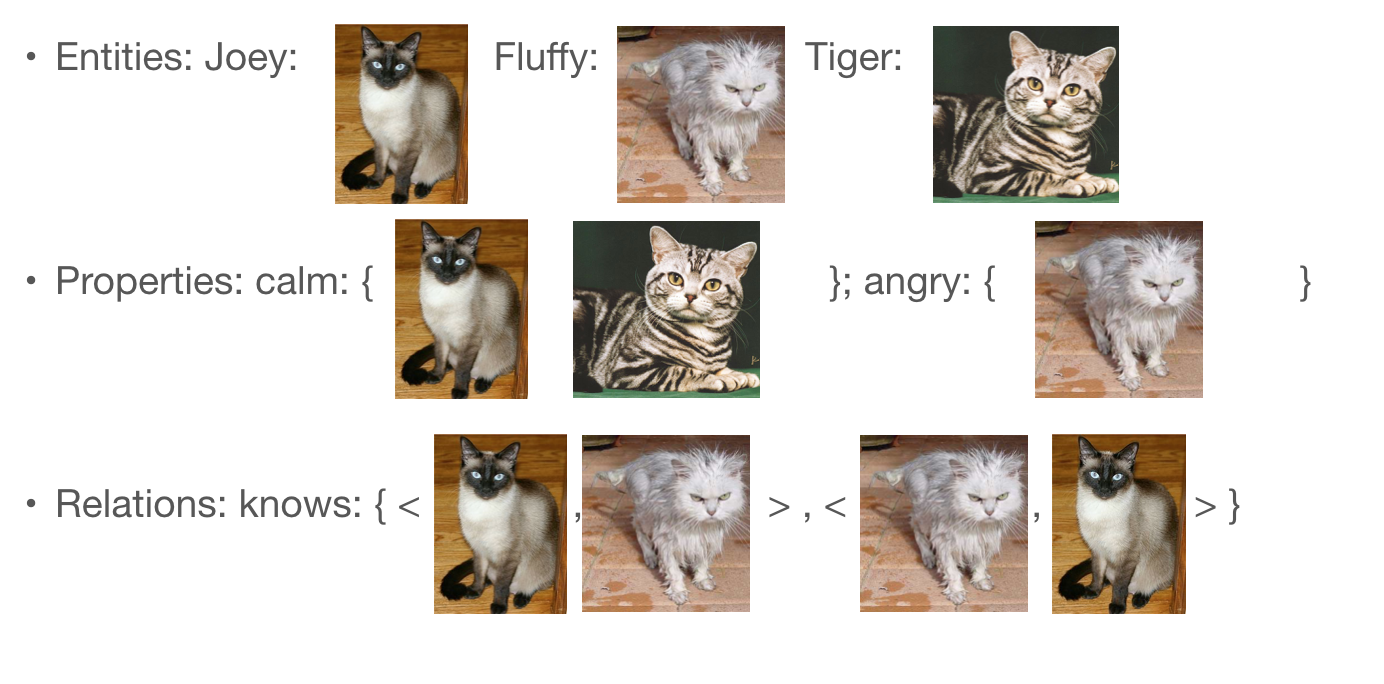
\includegraphics[width=\textwidth]{figures/cats1}
\end{frame}

\begin{frame}{Model theoretic semantics (denotations)}
  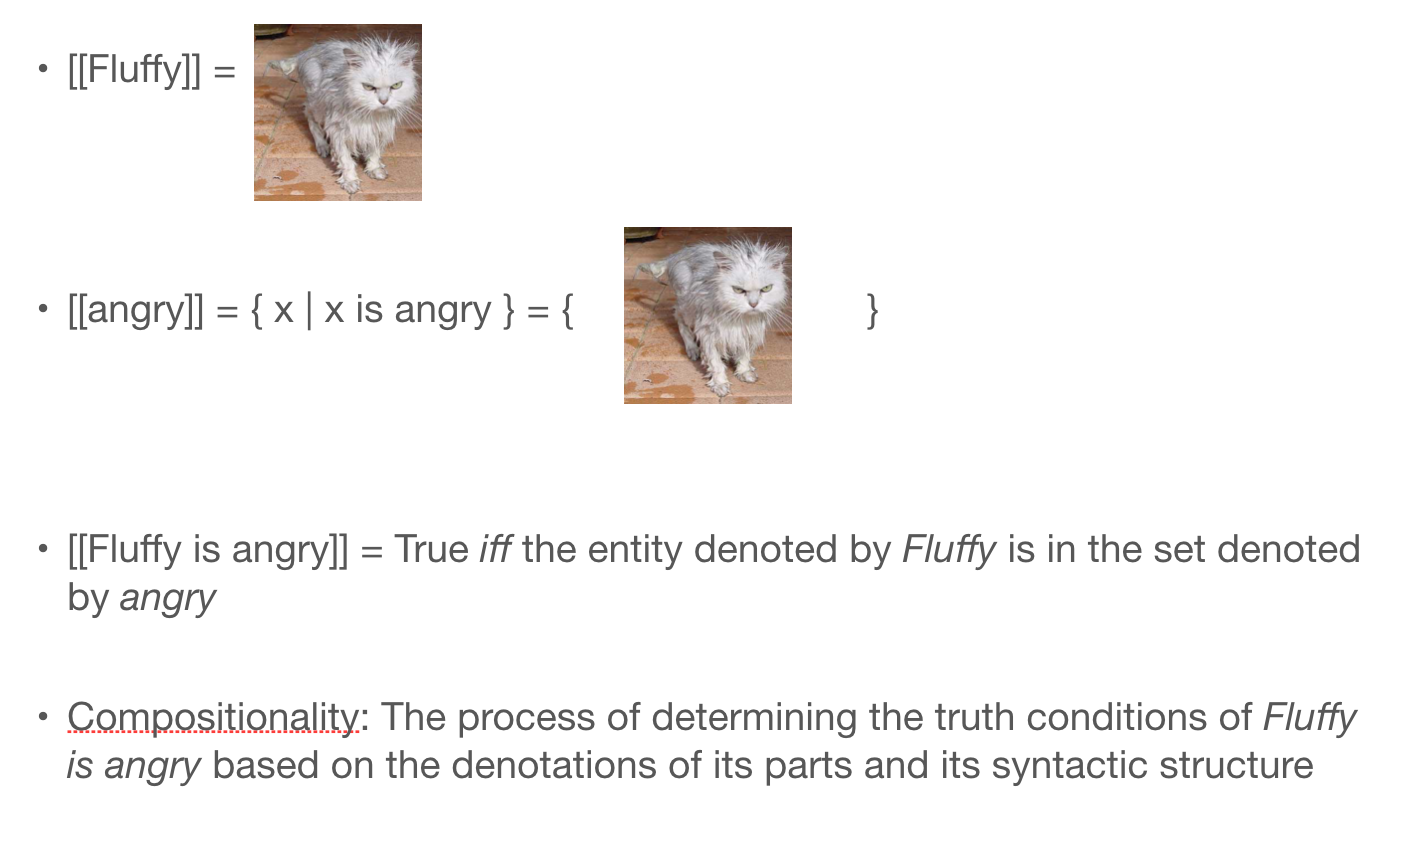
\includegraphics[width=\textwidth]{figures/cats2}
\end{frame}

\begin{frame}{Logical vocabulary gets special treatment}
  \begin{itemize}
  \item Fluffy is angry and Joey is not angry.
    \begin{itemize}
    \item What does {\it and} mean?
    \item What does {\it not} mean?
    \end{itemize}
  \item Every cat is angry.
    \begin{itemize}
    \item What does {\it cat} mean?  
    \item What does {\it every} mean?
    \end{itemize}
  \item Is the division into logical and non-logical vocabulary an
    inherent property of language or an artifact of the system of
    meaning representation?
  \end{itemize}
\end{frame}

\begin{frame}{Quantifiers}
  \begin{itemize}
  \item The semantic type of a quantifier is a relation between sets,
    called the restriction and body (or scope) of the quantifier
  \item $[\![every]\!]$ \{ $<$P,Q$>$ $\vert$ P $\subseteq$ Q\}
  \item $[\![$every cat is angry$]\!]$ is True iff 
    \{ x $\vert$ x is a cat \} $\subseteq$ \{ y $\vert$ y is angry \}
  \item $[\![some]\!]$ \{ $<$P,Q$>$ $\vert$ P $\cap$ Q $\neq$ $\emptyset$\}
  \item $[\![$some cat is angry$]\!]$ is True iff
    \{ x $\vert$ x is a cat \} $\cap$ \{ y $\vert$ y is angry \} $\neq$ $\emptyset$
  \item $[\![many]\!]$ ?
  \end{itemize}
\end{frame}

\section{Lambda calculus}

\begin{frame}{Partial evaluation for FOL: Lambda calculus}
  \begin{itemize}
  \item Basic idea: pass around partially evaluated functions
  \item feed them to other functions as arguments
  \item e.g.\ $f: y = x + 2$
  \item plug in $x = 3$, evaluate to 5
  \item or: $f: z = y*(x+2)$
  \item plug in $x = 3$, evaluate to $f: z = 3y$
  \item then can plug in y = 2 and evaluate to 6
  \end{itemize}
\end{frame}

\begin{frame}{Lambda calculus for semantics}
  \begin{itemize}
  \item Used to evaluate FOL expressions in a compositional manner
  \item e.g.\ constituent by constituent
  \item A constituent does not necessarily have a truth value:
  \item gave(Kim,book,x)
  \item need to hold on to a partially evaluated constituent
  \item Converting multi-argument predicates to sequences of single-argument predicates
  \item Incrementally accumulates multiple arguments spread over different parts of the tree
  \end{itemize}
\end{frame}

\begin{frame}{Lambda calculus}
  \begin{itemize}
  \item Form: $\lambda$ + Variable + FOL expression
  \item $\lambda x.P(x)$ (evaluating the expression with respect to $x$)
  \item $\lambda x.P(x)(A) \rightarrow P(A)$ ($\lambda$-reduction; binding a formal parameter to a concrete term)
  \item $\lambda x.\lambda y.Near(x,y)$
  \item $\lambda x.\lambda y.Near(x,y)(Moscow)$
  \item $\lambda y.Near(Moscow,y)$
  \item $\lambda y.Near(Moscow,y)(Center)$
  \item $Near(Moscow,Center)$
  \end{itemize}
\end{frame}

\section{Computational semantics}

\begin{frame}{Computational semantics desiderata (J\&M)}
  \begin{itemize}
  \item Verifiability: We must be able to compare the representation to a knowledge base
  \item Lack of ambiguity: A semantic representation should have just one interpretation
  \item Canonical form: A given interpretation should have just one representation
  \item Expressiveness: Must be able to adequately represent a wide range of expressions
  \end{itemize}
\end{frame}

\begin{frame}{Computational semantics desiderata (Copestake)}
  \begin{itemize}
  \item Expressive Adequacy: The framework must allow linguistic meanings to be expressed correctly
  \item Grammatical Compatibility: clear link to other kinds of grammatical information (most notably syntax)
  \item Computational Tractability: Process meanings, check semantic
    equivalence, express relationships between semantic
    representations straightforwardly
  \item Underspecifiability: Allow resolution of partial semantic representations
  \end{itemize}
\end{frame}

\begin{frame}{Computational semantics}
  \begin{itemize}
  \item Semantic parsing: mapping surface sentence to a semantic representation
  \item Should this representation be a structure?
  \item Sentence meaning: probably yes
  \item Speaker meaning: unclear
  \item (But sentence meaning is usually directly involved in speaker meaning)
  \end{itemize}
\end{frame}

\begin{frame}{Sentence vs. Speaker meaning (Grice 1968)}
  \begin{itemize}
  \item Through experience within our speech communities, we learn (and help create) shared linguistic conventions.
  \item These conventions support fairly consistent calculation of
    {\bf sentence meaning} by different speakers in the same
    community.
  \item The sentence meaning of an utterance (together with its form)
    serves as a clue which a listener can use to construct his/her
    representation of the speaker's {\bf speaker meaning}
  \end{itemize}
\end{frame}

\begin{frame}{Sentence vs. Speaker meaning}

  {\it Could you pass me the salt? -- No, I couldn't pass you the salt!}

  \vspace{1cm}

  \begin{itemize}
  \item Sentence meaning, but not speaker meaning, is compositional
  \item Systems attempting to understand speaker meaning directly from
    surface: resolve the same problems around grammatical structure
    for each task unlikely to scale
\end{itemize}
\end{frame}

\begin{frame}{Semantic compositionality}
  \begin{itemize}
  \item The meaning of the whole must be directly assembled from its parts
  \item E.g.\ {\it Agent/patient} information comes from the {\it subject/object constituents}
  \item The syntactico-semantic formalism must explicitly ensure such connections and assembly
  \end{itemize}
\end{frame}

\begin{frame}{Compositional layer and syntax-semantics interface}
  \begin{itemize}
  \item Predicate-argument structure
  \item Scope of negation and other operators
  \item Restriction of quantifiers
  \item Modality
  \item Tense/aspect/mood
  \item Information structure
  \item Discourse status of referents of NPs
  \item Politeness
  \end{itemize}
\end{frame}

\begin{frame}{Minimal Recursion Semantics (MRS)}
  \begin{itemize}
  \item An example of a compositional computational semantics approach
  \item Copestake et al. (2005)
  \item A semantic formalism (not a semantic theory)
  \end{itemize}

  \begin{center}
    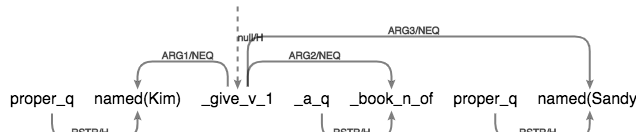
\includegraphics[width=.8\textwidth]{figures/dmrs}
    
    {\it Kim gave a book to Sandy}
  \end{center}
\end{frame}

\begin{frame}{Minimal Recursion Semantics (MRS)}

  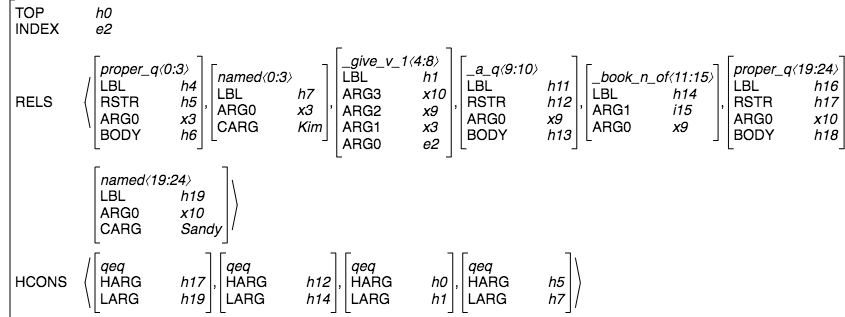
\includegraphics[width=\textwidth]{figures/mrs}

  \vspace{1cm}
  
  \centering
  {\it Kim gave a book to Sandy}
\end{frame}

\begin{frame}{Machine translation by transfer}
  \begin{itemize}
  \item Assuming a canonical form for semantic structure, we can generate sentences in one language given a semantic structure which was obtained by parsing a sentence in another language
  \item A {\bf symbolic} approach to MT
  \item Requires {\bf grammars} for both languages
  \item Ensures {\bf precision and grammaticality} of the translations
  \item Disadvantage: lack of {\bf robustness}: not every sentence will be translated.
  \end{itemize}
\end{frame}

\begin{frame}{MRS: MINIMAL recursion semantics}
  \begin{itemize}
  \item Syntactic structure may sometimes be irrelevant to the truth conditions
  \item {\it fierce black cat} vs {\it gato negro y feroz}
  \item with syntax insufficiently abstracted away, hard to do transfer
  \item the LFs produced by the two grammars will look different:
    
    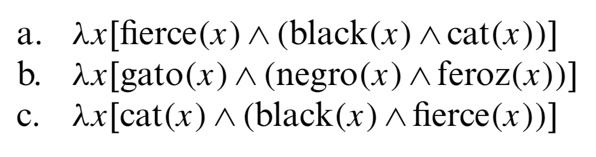
\includegraphics[width=0.8\textwidth]{figures/lfs}	
    
  \item $fierce(x) \wedge black(x) \wedge cat(x)$ -- solution?	
  \end{itemize}
\end{frame}

\begin{frame}{Flat semantics: quantifier problem}
  \begin{itemize}
  \item {\it Every white horse is old}
  \item every (x, white (x) $\wedge$ horse (x), old (x))
  \item Flat: every(x), horse(x), old(x), white(x)
  \item problem?
  \end{itemize}
\end{frame}

\begin{frame}{Flat semantics: quantifier problem}
  \begin{itemize}
  \item {\it Every white horse is old}
  \item every (x, white (x) $\wedge$ horse (x), old (x))
  \item Flat: every(x), horse(x), old(x), white(x)
  \item problem?
  \item {\it Every old horse is white}?
  \end{itemize}
\end{frame}

\begin{frame}{Quantifier scope}
  {\it Every dog chases some white cat}

  \vspace{0.7cm}

  \centering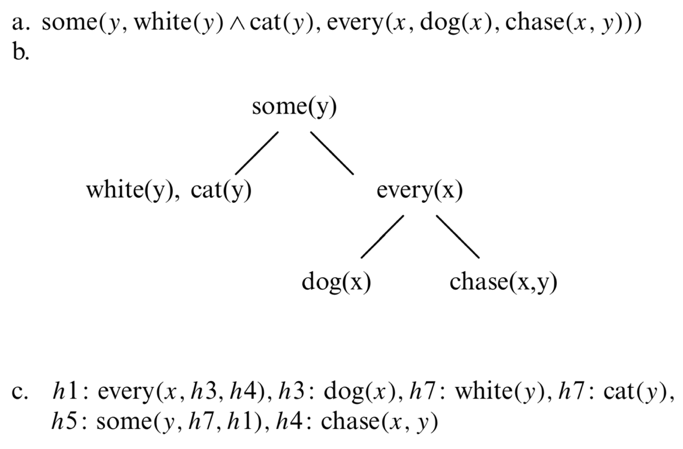
\includegraphics[width=\textwidth]{figures/scope1}
\end{frame}

\begin{frame}{Quantifier scope}
{\it Every dog chases some white cat}

\vspace{0.7cm}

\centering
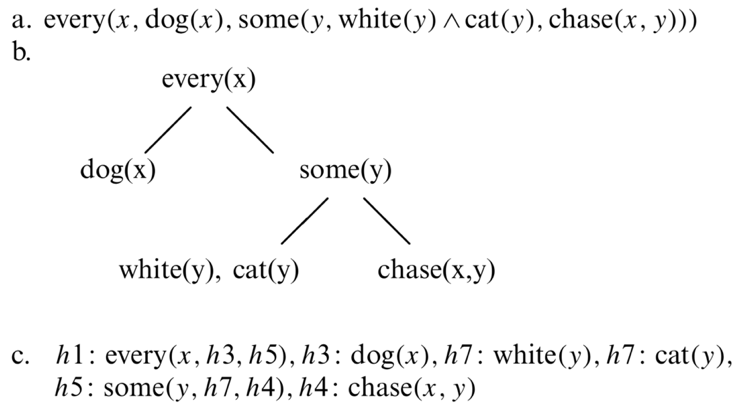
\includegraphics[width=\textwidth]{figures/scope2}
\end{frame}

\begin{frame}{Scope underspecification}
  \begin{minipage}{0.45\textwidth}
    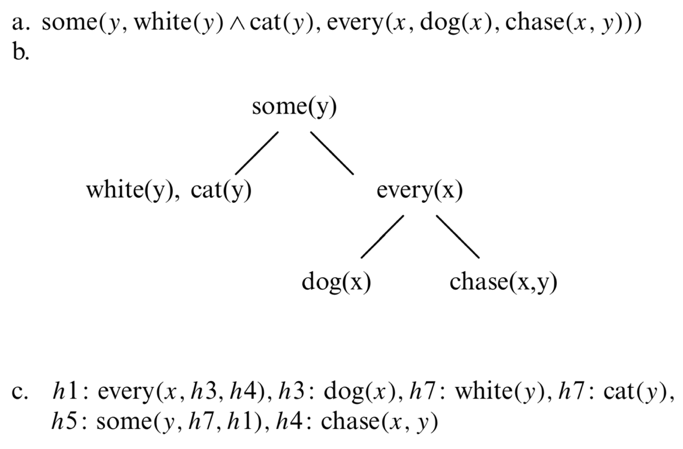
\includegraphics[height=0.4\textheight,width=\linewidth]{figures/scope1}
  \end{minipage}
  \begin{minipage}{0.45\textwidth}
    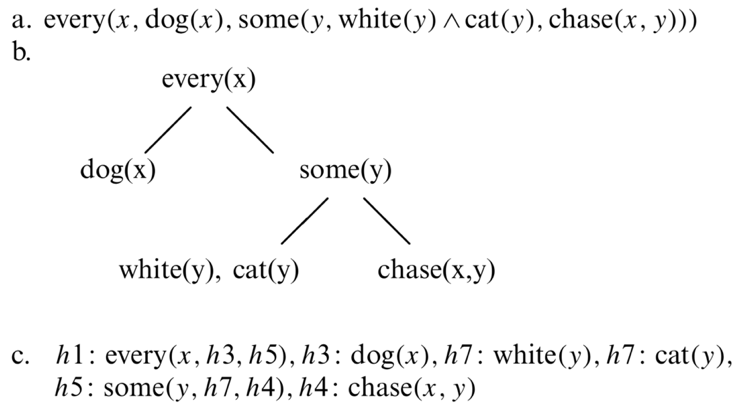
\includegraphics[height=0.4\textheight,width=\linewidth]{figures/scope2}
  \end{minipage}
  % \vspace{0.7cm}

  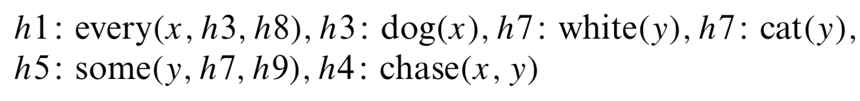
\includegraphics[width=\textwidth]{figures/scope3}

  \begin{itemize}
  \item {\it Every dog chases some white cat}
  \item Can say EITHER h9=h1 OR h8-h5
\end{itemize}
\end{frame}

\section{Semantics in NLP}

\begin{frame}{NLP business with semantics}
  \begin{itemize}
  \item Construct knowledge base or model of the world
  \item Extract meaning representations from linguistic input
  \item Match input to world knowledge
  \item Produce replies/take action on the basis of the results
  \end{itemize}
\end{frame}


\begin{frame}{Semantics in NLP}
  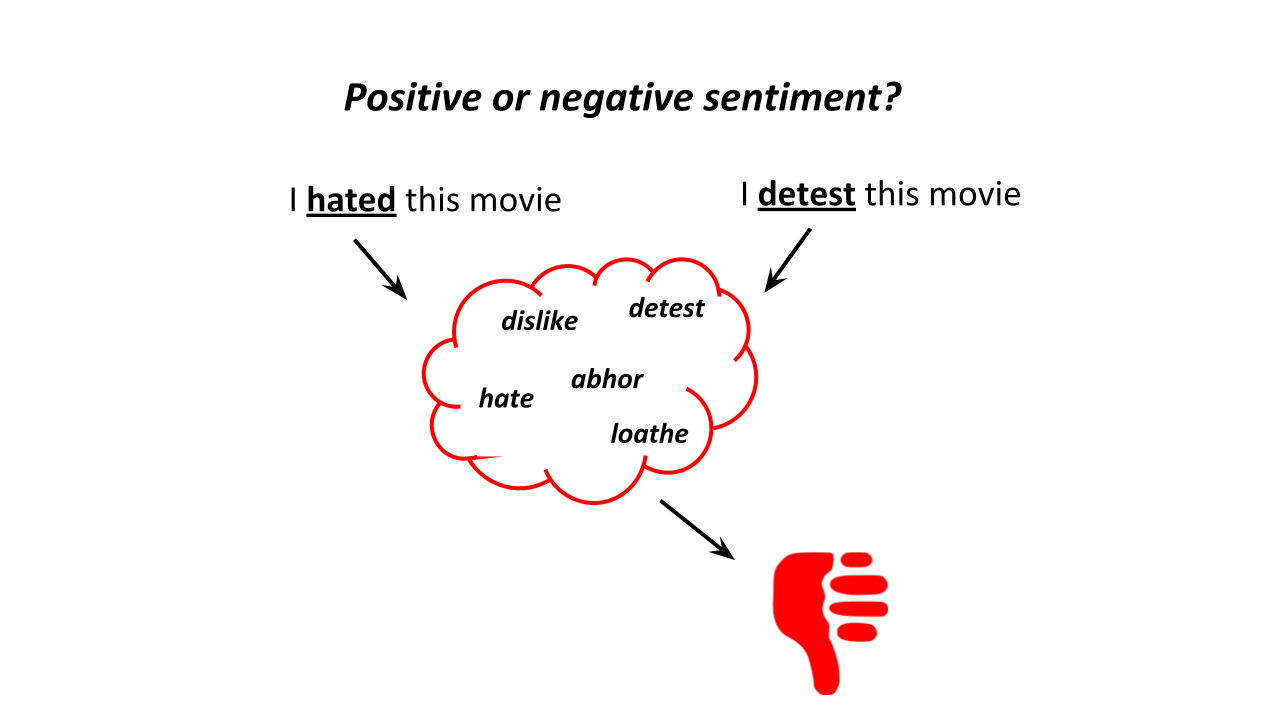
\includegraphics[height=0.5\textheight]{figures/sentiment}
  \vspace{0.4cm}
  
  \begin{itemize}
  \item Linguistic models, syntactic or semantic (or morphological...)
    tend to be too unwieldy for today's NLP
  \item NLP goals: perform well on a task, not necessarily precisely
    and not necessarily providing explanations
  \item Tacit expectation to map directly from {\it surface} to {\it
      speaker meaning}
  \end{itemize}
\end{frame}

\begin{frame}{Pre-vector space semantics in NLP}

  \begin{itemize}
  \item e.g.\ Abstract Meaning Representation (AMR; Banarescu et al., 2013)
  \item Note similarities with dependency parse
  \end{itemize}
  
  \vspace{0.4cm}

  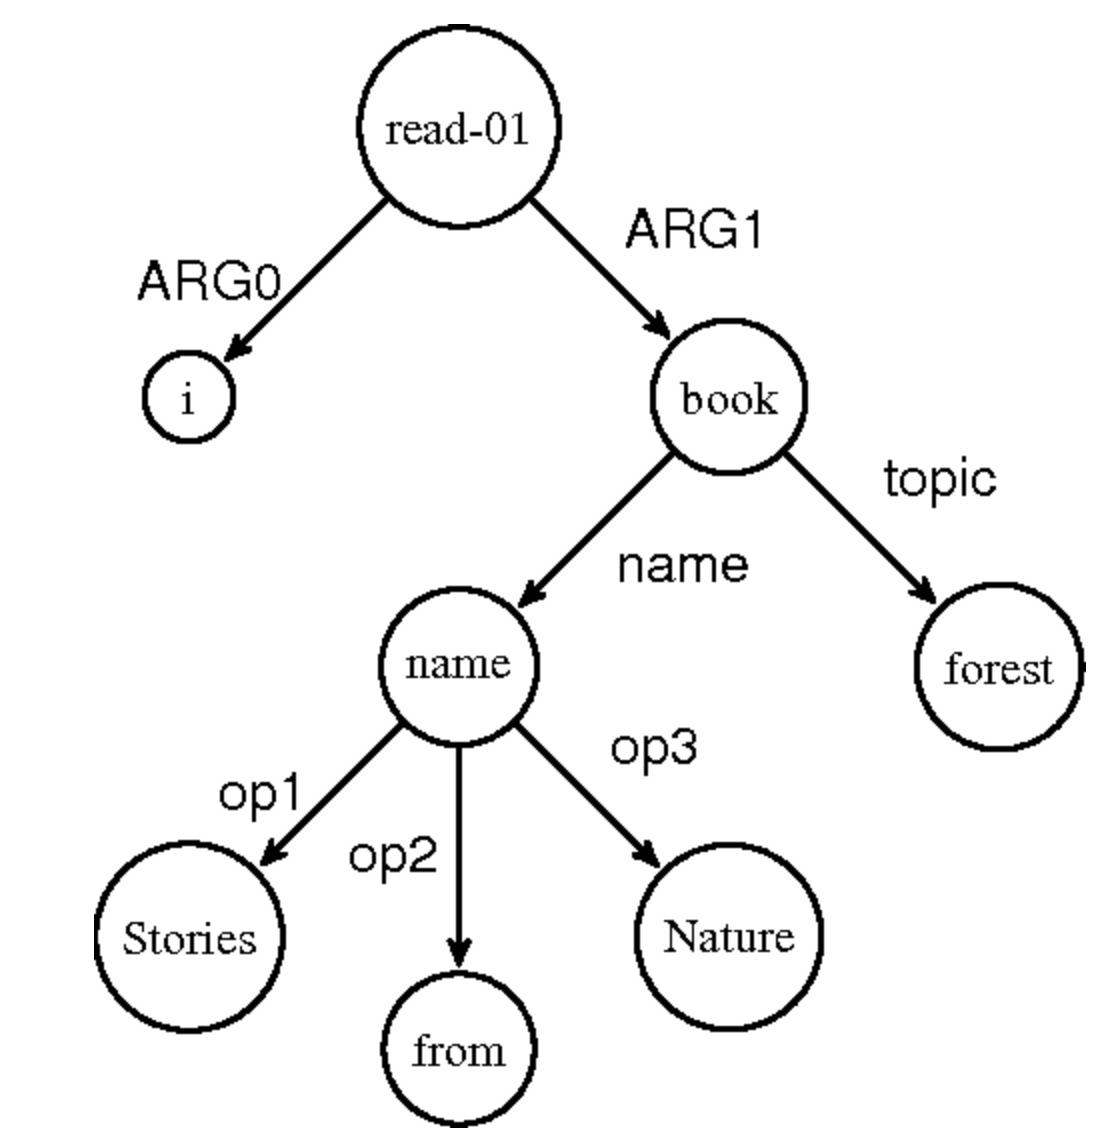
\includegraphics[height=0.7\textheight]{figures/amr}
\end{frame}

\begin{frame}{AMR: a widely adopted formalism}

  {\it "We describe Abstract Meaning Representation (AMR), a semantic
    representation language in which we are writing down the meanings
    of thousands of English sentences. We hope that a sembank of
    simple, whole-sentence semantic structures will spur new work in
    statistical natural language understanding and generation, like
    the Penn Treebank encouraged work on statistical parsing."}
  (Banarescu et al., 2013)
	
\end{frame}

\begin{frame}{Sembanks, Propbanks...}
  \begin{itemize}
  \item Representations like AMR can be stored in ``sembanks''
  \item Compare to treebanks
  \item Challenge: {\bf interannotator agreement}
    \begin{itemize}
    \item ...is a problem with treebanks, too, unless a grammar is used
    \item is even a bigger problem in sembanks
    \item role-labeling is more vague than syntactic structure
    \item e.g.\ what kind of granularity?
    \end{itemize}
  \item Familiar issues with overfitting
  \end{itemize}
\end{frame}

\begin{frame}{PropBank}
  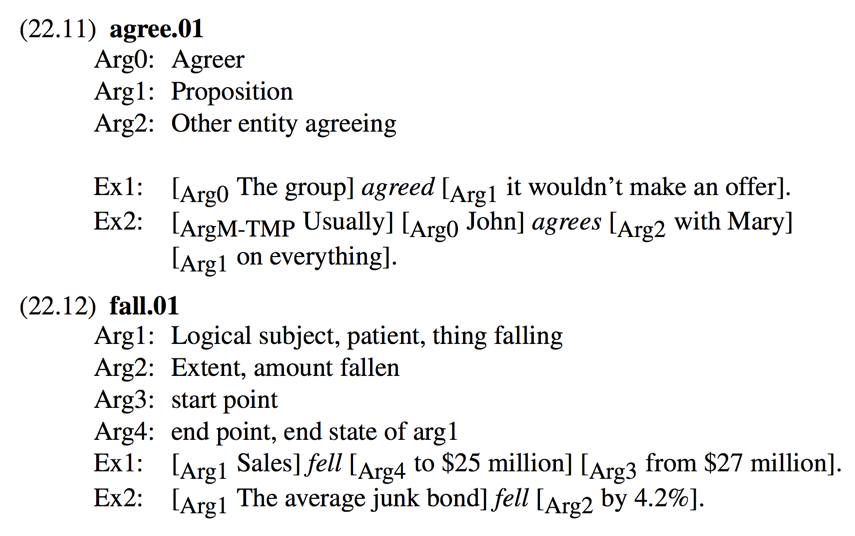
\includegraphics[width=\textwidth]{figures/propbank}
\end{frame}

\begin{frame}{AI, robotics and grounded reasoning}

  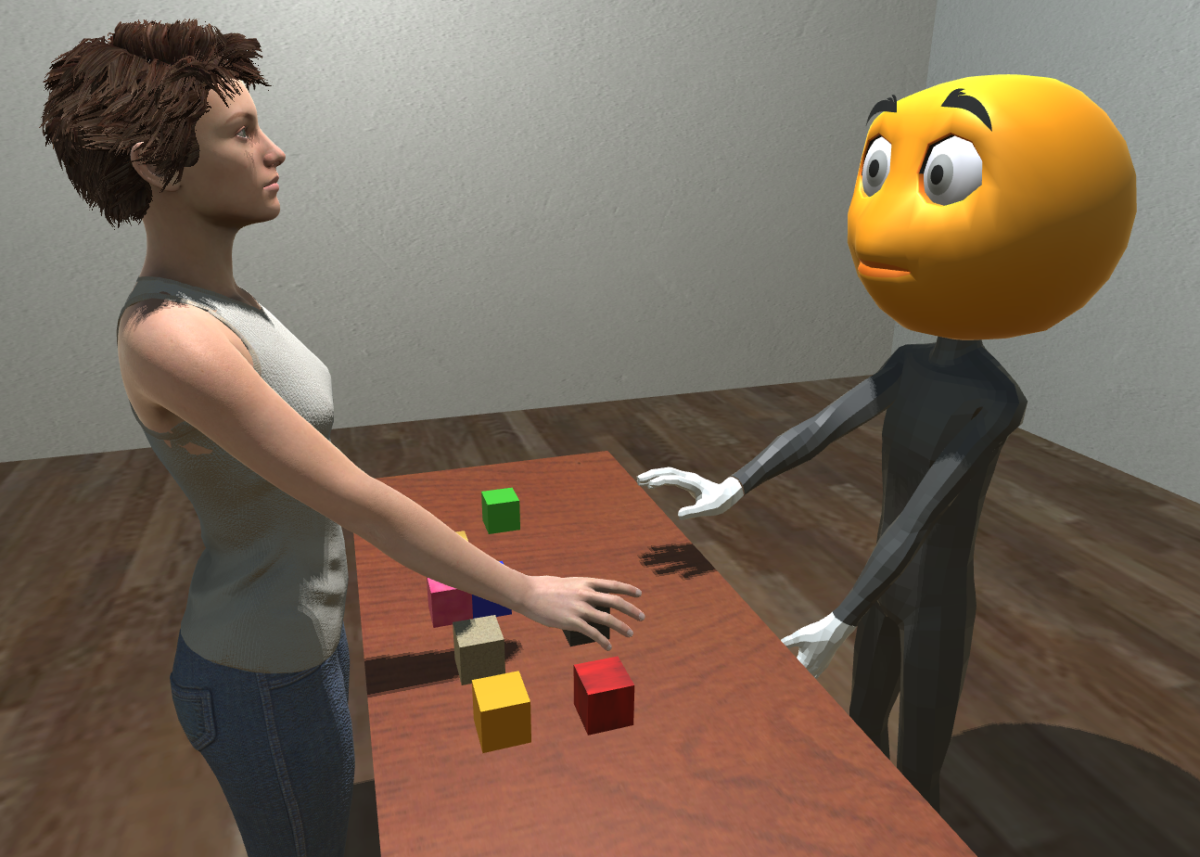
\includegraphics[height=0.7\textheight]{figures/krishnaswamy}

  \begin{itemize}
  \item {\it There is exactly one yellow object touching the wall}
  \item (object-count-equals (yellow (touch-wall all-objects)) 1)
  \item {\it natural} language?..
  \end{itemize}
\end{frame}

\begin{frame}{Vector space semantics (next lecture)}
  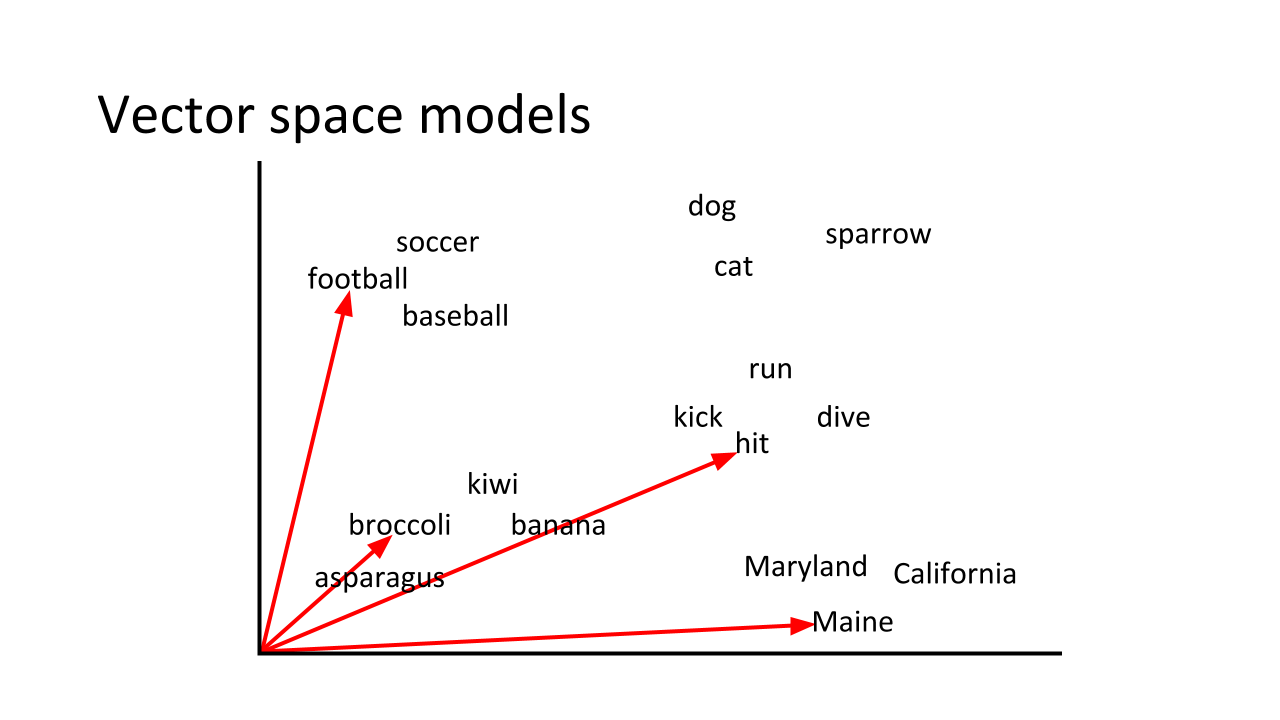
\includegraphics[height=0.6\textheight]{figures/vector-space}
  \begin{itemize}
  \item The core of today's NLP
  \item Are word vectors semantic representations?
  \item Yes, but not necessarily compositional
  \end{itemize}
\end{frame}

\end{document}

%%% Local Variables:
%%% mode: latex
%%% TeX-master: t
%%% End:
